\chapter{CONFIABILIDADE DO SISTEMA}
\label{chap:conf}
A fim de verificar-se a confiabilidade do sistema, foi realizado o levantamento de cada componente que constitui o manipulador robótico e o estudo detalhado das prováveis falhas. Para isso, foi utilizado o \textit{\acs{FMECA}} com o propósito de analisar cada sub-sistema, como pode ser visto nas tabelas da seção \ref{sec:fmeca}. 

Na seção \ref{sec:fta} foi desenvolvida a análise da árvore de falhas do sistema, método que permite através de um processo lógico dedutivo chegar-se às causas básicas de um problema de proporções maiores.

%------------------------------------------------------------------
\section{Análise dos modos e efeitos de falhas}
\label{sec:fmeca}
  Nas Tabelas \ref{tab:sistema_potencia}, \ref{tab:sistema_aquisicao}, \ref{tab:sistema_estrutural}, \ref{tab:sistema_atuacao} e \ref{tab:sistema_processamento}  estão representadas informações referentes ao estudo sistemático e estrutura das falhas potenciais para os sub-sistemas de potência, de aquisição, estrutural, de atuação e de processamento, respectivamente. 



  \begin{table}[H]
    \caption{ \textit{FMECA} do sub-sistema de potência}
    \begin{adjustbox}{max width=\textwidth}
    \begin{tabular}{|c|c|c|c|c|c|c|c|c|}
    \hline
    \rowcolor[HTML]{EFEFEF} 
    \multicolumn{9}{|c|}{\cellcolor[HTML]{EFEFEF}\textbf{Análise do Tipo e Efeito de Falha}} \\ \hline
    \multicolumn{9}{|c|}{\textbf{Sub-sistema de potência}} \\ \hline
    \rowcolor[HTML]{EFEFEF} 
    \textbf{Função(ões)} &
      \textbf{\begin{tabular}[c]{@{}c@{}}Modo(s) de falha\\ em potencial\end{tabular}} &
      \textbf{\begin{tabular}[c]{@{}c@{}}Efeito(s) potencial(is)\\ da falha\end{tabular}} &
      \textbf{S} &
      \textbf{\begin{tabular}[c]{@{}c@{}}Causa(s)\\ potenciais\end{tabular}} &
      \textbf{O} &
      \textbf{D} &
      \textbf{C} &
      \textbf{\begin{tabular}[c]{@{}c@{}}Ação(ões) \\ recomendada(s)\end{tabular}} \\ \hline
     &
       &
      \begin{tabular}[c]{@{}c@{}}Comprometimento dos\\  dados transmitidos\end{tabular} &
      6 &
      Fissura dos fios &
      3 &
      5 &
      90 &
       \\ \cline{3-8}
    \multirow{-2}{*}{\begin{tabular}[c]{@{}c@{}}Transmissão \\ de dados\end{tabular}} &
      \multirow{-2}{*}{\begin{tabular}[c]{@{}c@{}}Incapacidade de \\ transmissão\\de dados\end{tabular}} &
      \begin{tabular}[c]{@{}c@{}}Perda da capacidade \\ de transmissão \\ de dados\end{tabular} &
      8 &
      \begin{tabular}[c]{@{}c@{}}Desgaste causado \\ pelo tempo\end{tabular} &
      2 &
      1 &
      16 &
      \multirow{-2}{*}{\begin{tabular}[c]{@{}c@{}}Manutenções \\ preventivas\end{tabular}} \\ \hline
     &
       &
      \begin{tabular}[c]{@{}c@{}}Perda da capacidade\\de transmissão de energia\end{tabular} &
      8 &
      \begin{tabular}[c]{@{}c@{}}Derretimento por \\ temperatura elevada\end{tabular} &
      1 &
      1 &
      8 &
      \begin{tabular}[c]{@{}c@{}}Manutenções \\ preventivas\end{tabular} \\ \cline{3-9} 
    \multirow{-2}{*}{\begin{tabular}[c]{@{}c@{}}Transmissão \\ de energia\end{tabular}} &
      \multirow{-2}{*}{\begin{tabular}[c]{@{}c@{}}Incapacidade de\\transmissão de energia\end{tabular}} &
      \begin{tabular}[c]{@{}c@{}}Má qualidade da \\ energia transmitida\end{tabular} &
      6 &
      Torção dos fios &
      3 &
      5 &
      90 &
      \multicolumn{1}{l|}{} \\ \hline
     &
       &
       &
       &
      \begin{tabular}[c]{@{}c@{}}Má conexão \\ com fonte de tensão\end{tabular} &
      3 &
      6 &
      162 &
      \begin{tabular}[c]{@{}c@{}}Verificar conexão\\  com fonte\end{tabular} \\ \cline{5-9} 
    \multirow{-2}{*}{\begin{tabular}[c]{@{}c@{}}Alimentação\\ do sistema\end{tabular}} &
      \multirow{-2}{*}{\begin{tabular}[c]{@{}c@{}}Incapacidade \\ em fornecer energia\end{tabular}} &
      \multirow{-2}{*}{\begin{tabular}[c]{@{}c@{}}Não energização\\  do sistema\end{tabular}} &
      \multirow{-2}{*}{9} &
      \begin{tabular}[c]{@{}c@{}}Desgaste nas soldas \\ causado pelo tempo\end{tabular} &
      4 &
      7 &
      252 &
      \begin{tabular}[c]{@{}c@{}}Verificar continuidade\\ na placa do circuito\end{tabular} \\ \hline
    \end{tabular}
    \end{adjustbox}
    \legend{Fonte: Autoria própria.}
    \label{tab:sistema_potencia}
    \end{table}



\begin{table}[H]
  \caption{ \textit{FMECA} do sub-sistema aquisição}
  \begin{adjustbox}{max width=\textwidth}
  \begin{tabular}{|c|c|c|c|c|c|c|c|c|}
  \hline
  \rowcolor[HTML]{EFEFEF}
  \multicolumn{9}{|c|}{\cellcolor[HTML]{EFEFEF}\textbf{Análise do Tipo e Efeito de Falha}} \\ \hline
  \rowcolor[HTML]{FFFFFF} 
  \multicolumn{9}{|c|}{\cellcolor[HTML]{FFFFFF}\textbf{Sub-sistema de aquisição}} \\ \hline
  \rowcolor[HTML]{EFEFEF} 
  \textbf{Função(ões)} & \textbf{\begin{tabular}[c]{@{}c@{}}Modo(s) de falha \\ em potencial\end{tabular}} & \textbf{\begin{tabular}[c]{@{}c@{}}Efeito(s) potencial(is) \\ da falha\end{tabular}} & \textbf{S} & \textbf{\begin{tabular}[c]{@{}c@{}}Causa(s) \\ potenciais\end{tabular}} & \textbf{O} & \textbf{D} & \textbf{C} & \textbf{\begin{tabular}[c]{@{}c@{}}Ação(ões) \\ recomendada(s)\end{tabular}} \\ \hline
  \rowcolor[HTML]{FFFFFF} 
  \cellcolor[HTML]{FFFFFF} & \begin{tabular}[c]{@{}c@{}}Incapacidade de \\ obter dados visuais\end{tabular} & \cellcolor[HTML]{FFFFFF} & \cellcolor[HTML]{FFFFFF} & \begin{tabular}[c]{@{}c@{}}Obstrução do campo \\ de visão da câmera\end{tabular} & 2 & 1 & 16 & \cellcolor[HTML]{FFFFFF} \\ \cline{2-2} \cline{5-8}
  \rowcolor[HTML]{FFFFFF} 
  \cellcolor[HTML]{FFFFFF} & \cellcolor[HTML]{FFFFFF} & \cellcolor[HTML]{FFFFFF} & \cellcolor[HTML]{FFFFFF} & \begin{tabular}[c]{@{}c@{}}Baixa visibilidade \\ do ambiente\end{tabular} & 2 & 5 & 80 & \cellcolor[HTML]{FFFFFF} \\ \cline{5-8}
  \rowcolor[HTML]{FFFFFF} 
  \cellcolor[HTML]{FFFFFF} & \multirow{-2}{*}{\cellcolor[HTML]{FFFFFF}\begin{tabular}[c]{@{}c@{}}Ruptura da estrutura \\ de fixação da câmera\end{tabular}} & \multirow{-3}{*}{\cellcolor[HTML]{FFFFFF}\begin{tabular}[c]{@{}c@{}}Perda da capacidade \\ de obter dados visuais\end{tabular}} & \multirow{-3}{*}{\cellcolor[HTML]{FFFFFF}8} & \begin{tabular}[c]{@{}c@{}}Calibração incorreta \\ da câmera\end{tabular} & 3 & 1 & 24 & \multirow{-3}{*}{\cellcolor[HTML]{FFFFFF}\begin{tabular}[c]{@{}c@{}}Verificar condições do\\ ambiente antes das missões\end{tabular}} \\ \cline{2-9} 
  \rowcolor[HTML]{FFFFFF} 
  \cellcolor[HTML]{FFFFFF} & \cellcolor[HTML]{FFFFFF} & \cellcolor[HTML]{FFFFFF} & \cellcolor[HTML]{FFFFFF} & Set-up incorreto & 2 & 7 & 84 & \cellcolor[HTML]{FFFFFF} \\ \cline{5-8}
  \rowcolor[HTML]{FFFFFF} 
  \multirow{-5}{*}{\cellcolor[HTML]{FFFFFF}\begin{tabular}[c]{@{}c@{}}Aquisição de \\ dados visuais\end{tabular}} & \multirow{-2}{*}{\cellcolor[HTML]{FFFFFF}\begin{tabular}[c]{@{}c@{}}Coleta de dados \\ inconsistentes ou insuficientes\end{tabular}} & \multirow{-2}{*}{\cellcolor[HTML]{FFFFFF}\begin{tabular}[c]{@{}c@{}}Comprometimento \\ dos dados\end{tabular}} & \multirow{-2}{*}{\cellcolor[HTML]{FFFFFF}6} & \begin{tabular}[c]{@{}c@{}}Falha no canal \\ de comunicação\end{tabular} & 4 & 7 & 168 & \multirow{-2}{*}{\cellcolor[HTML]{FFFFFF}\begin{tabular}[c]{@{}c@{}}Verificar cabeamento\\ do sistema\end{tabular}} \\ \hline
  \end{tabular}
\end{adjustbox}
\legend{Fonte: Autoria própria.}
\label{tab:sistema_aquisicao}
  \end{table}

      \begin{table}[H]
      \caption{ \textit{FMECA} do sub-sistema estrutural}
      \begin{adjustbox}{max width=\textwidth}
        \begin{tabular}{|c|c|c|l|c|l|l|c|c|}
        \hline
        \rowcolor[HTML]{EFEFEF} 
        \multicolumn{9}{|c|}{\cellcolor[HTML]{EFEFEF}\textbf{Análise do Tipo e Efeito de Falha}} \\ \hline
        \multicolumn{9}{|c|}{\textbf{Sub-sistema estrutural}} \\ \hline
        \rowcolor[HTML]{EFEFEF} 
        \textbf{Função(ões)} &
          \textbf{\begin{tabular}[c]{@{}c@{}}Modo(s) de falha\\ em potencial\end{tabular}} &
          \textbf{\begin{tabular}[c]{@{}c@{}}Efeito(s) potencial(is)\\ da falha\end{tabular}} &
          \textbf{S} &
          \textbf{\begin{tabular}[c]{@{}c@{}}Causa(s)\\ potenciais\end{tabular}} &
          \textbf{O} &
          \textbf{D} &
          \textbf{C} &
          \textbf{\begin{tabular}[c]{@{}c@{}}Ação(ões)\\ \\ recomendada(s)\end{tabular}} \\ \hline
         &
           &
           &
           &
          \begin{tabular}[c]{@{}c@{}}Excesso de \\ peso aplicado\end{tabular} &
          2 &
          1 &
          16 &
           \\ \cline{5-8}
         &
           &
          \multirow{-2}{*}{Ruptura do conector} &
          \multirow{-2}{*}{8} &
          \begin{tabular}[c]{@{}c@{}}Desgaste \\ pelo tempo\end{tabular} &
          2 &
          5 &
          80 &
          \multirow{-2}{*}{\begin{tabular}[c]{@{}c@{}}Verificar a\\ fabricação da peça\end{tabular}} \\ \cline{3-9} 
         &
           &
           &
           &
          \begin{tabular}[c]{@{}c@{}}Set-up \\ incorreto\end{tabular} &
          4 &
          6 &
          144 &
           \\ \cline{5-8}
        \multirow{-4}{*}{\begin{tabular}[c]{@{}c@{}}Ligar o frame \\ ao perfil de \\ alumínio\end{tabular}} &
          \multirow{-4}{*}{\begin{tabular}[c]{@{}c@{}}Incapacidade de\\  sustentar o perfil\end{tabular}} &
          \multirow{-2}{*}{Trinca do conector} &
          \multirow{-2}{*}{6} &
          \begin{tabular}[c]{@{}c@{}}Defeito de \\ fabricação\end{tabular} &
          5 &
          6 &
          180 &
          \multirow{-2}{*}{\begin{tabular}[c]{@{}c@{}}Verificar as \\ condições de peso aplicadas\end{tabular}} \\ \hline
         &
          \begin{tabular}[c]{@{}c@{}}Danificação \\ estrutural\end{tabular} &
          Ruptura do perfil &
          8 &
          Sobrecarga &
          2 &
          4 &
          64 &
          \begin{tabular}[c]{@{}c@{}}Cuidado no \\ manuseamento \\ dos perfis\end{tabular} \\ \cline{2-9} 
        \multirow{-2}{*}{\begin{tabular}[c]{@{}c@{}}Compor\\ estrutura mecânica\end{tabular}} &
          \begin{tabular}[c]{@{}c@{}}Folga entre \\ conexões\end{tabular} &
          Empeno do perfil &
          6 &
          Colisão &
          4 &
          2 &
          48 &
          \begin{tabular}[c]{@{}c@{}}Definir \\ área de trabalho\end{tabular} \\ \hline
        \end{tabular}
        \end{adjustbox}
        \legend{Fonte: Autoria própria.}
        \label{tab:sistema_estrutural}
        \end{table}



        \begin{table}[H]
          \caption{ \textit{FMECA} do sub-sistema de atuação}
          \begin{adjustbox}{max width=\textwidth}
           \begin{tabular}{|c|c|c|c|c|c|c|c|c|}
              \hline
              \rowcolor[HTML]{EFEFEF} 
              \multicolumn{9}{|c|}{\cellcolor[HTML]{EFEFEF}\textbf{Análise do Tipo e Efeito de Falha}} \\ \hline
              \multicolumn{9}{|c|}{\textbf{Sub-sistema de atuação}} \\ \hline
              \rowcolor[HTML]{EFEFEF} 
              \textbf{Função(ões)} &
                \textbf{\begin{tabular}[c]{@{}c@{}}Modo(s) de falha\\ em potencial\end{tabular}} &
                \textbf{\begin{tabular}[c]{@{}c@{}}Efeito(s) potencial(is)\\ da falha\end{tabular}} &
                \textbf{S} &
                \textbf{\begin{tabular}[c]{@{}c@{}}Causa(s)\\ potenciais\end{tabular}} &
                \textbf{O} &
                \textbf{D} &
                \textbf{C} &
                \textbf{\begin{tabular}[c]{@{}c@{}}Ação(ões)\\ recomendada(s)\end{tabular}} \\ \hline
              \begin{tabular}[c]{@{}c@{}}Movimentação \\ do manipulador\end{tabular} &
                \begin{tabular}[c]{@{}c@{}}Rotação inconsistente \\ com o desejado\end{tabular} &
                \begin{tabular}[c]{@{}c@{}}Perda de desempenho \\ (velocidade; controle)\end{tabular} &
                6 &
                \begin{tabular}[c]{@{}c@{}}Emperramento \\ parcial\end{tabular} &
                4 &
                6 &
                144 &
                \begin{tabular}[c]{@{}c@{}}Inspeções \\ periódicas\end{tabular} \\ \hline
               &
                Curto circuito &
                Parada do motor &
                8 &
                \begin{tabular}[c]{@{}c@{}}Cabeamento \\ incorreto\end{tabular} &
                2 &
                5 &
                80 &
                 \\ \cline{2-8}
               &
                Perda de comunicação &
                 &
                 &
                 &
                 &
                 &
                 &
                 \\ \cline{2-2}
              \multirow{-3}{*}{\begin{tabular}[c]{@{}c@{}}Fornecer o torque\\  mínimo de sustentação\end{tabular}} &
                Tensão insuficiente &
                \multirow{-2}{*}{Perda de desempenho} &
                \multirow{-2}{*}{6} &
                \multirow{-2}{*}{\begin{tabular}[c]{@{}c@{}}Falha na \\ alimentação\end{tabular}} &
                \multirow{-2}{*}{4} &
                \multirow{-2}{*}{5} &
                \multirow{-2}{*}{120} &
                \multirow{-3}{*}{\begin{tabular}[c]{@{}c@{}}Medir corrente\\  nos terminais\end{tabular}} \\ \hline
              \end{tabular}
              \end{adjustbox}
              \legend{Fonte: Autoria própria.}
              \label{tab:sistema_atuacao}
              \end{table}


              \begin{table}[H]
                \caption{ \textit{FMECA} do sub-sistema de processamento}
                \begin{adjustbox}{max width=\textwidth}
                \begin{tabular}{|c|c|c|c|c|c|c|c|c|}
                \hline
                \rowcolor[HTML]{EFEFEF} 
                \multicolumn{9}{|c|}{\cellcolor[HTML]{EFEFEF}\textbf{Análise do Tipo e Efeito de Falha}} \\ \hline
                \multicolumn{9}{|c|}{\textbf{Sub-sistema de processamento}} \\ \hline
                \rowcolor[HTML]{EFEFEF} 
                \textbf{Função(ões)} &
                  \textbf{\begin{tabular}[c]{@{}c@{}}Modo(s) de falha\\ em potencial\end{tabular}} &
                  \textbf{\begin{tabular}[c]{@{}c@{}}Efeito(s) potencial(is)\\ da falha\end{tabular}} &
                  \textbf{S} &
                  \textbf{\begin{tabular}[c]{@{}c@{}}Causa(s)\\ potenciais\end{tabular}} &
                  \textbf{O} &
                  \textbf{D} &
                  \textbf{C} &
                  \textbf{\begin{tabular}[c]{@{}c@{}}Ação(ões) \\ recomendada(s)\end{tabular}} \\ \hline
                 &
                   &
                   &
                   &
                  \begin{tabular}[c]{@{}c@{}}Queima/ danificação \\ de componentes\end{tabular} &
                  3 &
                  8 &
                  216 &
                  \begin{tabular}[c]{@{}c@{}}Manutenção \\ preditiva\end{tabular} \\ \cline{5-9} 
                 &
                   &
                   &
                   &
                  \begin{tabular}[c]{@{}c@{}}Falha no sistema\\ operacional\end{tabular} &
                  2 &
                  8 &
                  144 &
                  \begin{tabular}[c]{@{}c@{}}Executar teste de \\ verificação do software\end{tabular} \\ \cline{5-9} 
                 &
                   &
                   &
                   &
                  \begin{tabular}[c]{@{}c@{}}Falha na porta de \\ comunicação\end{tabular} &
                  2 &
                  2 &
                  36 &
                  \begin{tabular}[c]{@{}c@{}}Exectutar teste de entrada\\ e saída de dados com \textit{NUC}\end{tabular} \\ \cline{5-9} 
                \multirow{-4}{*}{\begin{tabular}[c]{@{}c@{}}Processamento dos\\ dados\end{tabular}} &
                  \multirow{-4}{*}{\begin{tabular}[c]{@{}c@{}}Não processamento dos \\ dados do sistema principal\end{tabular}} &
                  \multirow{-4}{*}{Não funcionamento} &
                  \multirow{-4}{*}{9} &
                  \begin{tabular}[c]{@{}c@{}}Problemas de contato\\ elétrico\end{tabular} &
                  2 &
                  3 &
                  54 &
                  \begin{tabular}[c]{@{}c@{}}Inspeções periódicas\\ em bancada\end{tabular} \\ \hline
                \end{tabular}
                \end{adjustbox}
                \legend{Fonte: Autoria própria.}
                \label{tab:sistema_processamento}
                \end{table}
          

%------------------------------------------------------------------
%\section{Diagrama de blocos da Confiabilidade}
%\label{sec:diag}

%------------------------------------------------------------------
\section{Análise da árvore de falhas}
\label{sec:fta}

Na Figura \ref{fig:arvore_falha} encontra-se a árvore de falhas do sistema do manipulador JeRoTIMON. Observa-se que caso o manipulador não consiga realizar a tarefa de pressionar o botão, duas causas principais devem ser investigadas: a conexão entre as TF's, realizada a partir do pacote \textit{Bir Marker Localization}, ou o planejamento de trajetória, realizado pelo \textit{Moveit}. Para a primeira causa, devem ser verificadas as configurações do pacote e da câmera, bem como a orientação dos componentes envolvidos no processo de detecção. Já para solucionar os problemas correspondentes ao planejamento de trajetória, deve-se observar se a pose desejada está dentro do \textit{workspace} do manipulador e se o \textit{plugin} de cinemática inversa utilizado está sendo capaz de realizar as conversões necessárias para a pose desejada. 

\begin{figure}[H]
  \centering
  \caption{Árvore de falhas do sistema.}
  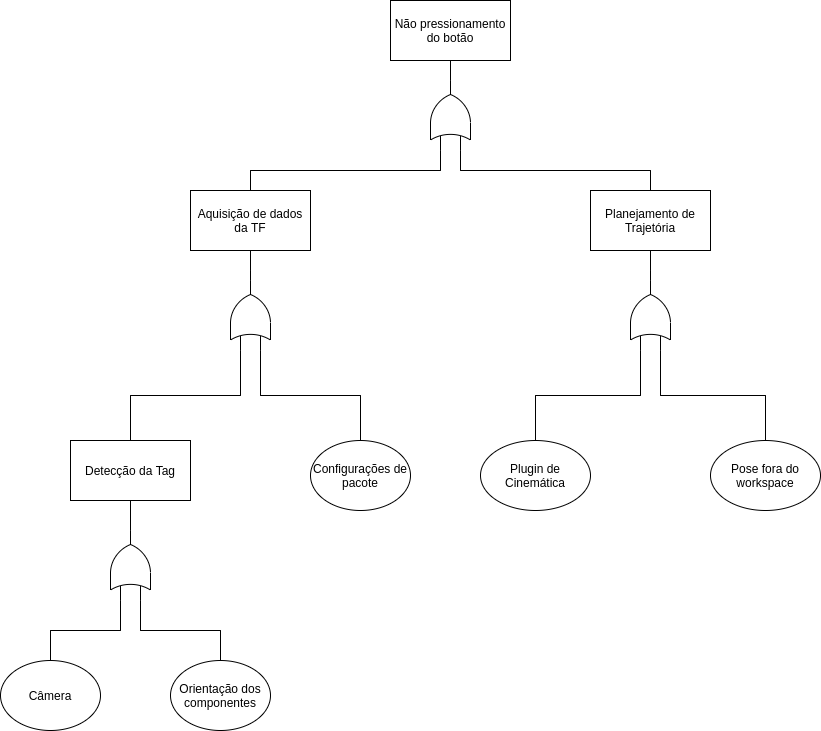
\includegraphics[scale=0.5]{images/arvore_falhas.png}
  \legend{Fonte: Autoria própria.}
  \label{fig:arvore_falha}
\end{figure}
